\chapter{ Energy Arbitrage, Imperfect Foresight }
\label{sec:imperfect_foresight}
\begin{wrapfigure}{r}{0.5\textwidth}
    \begin{center}
    \centering
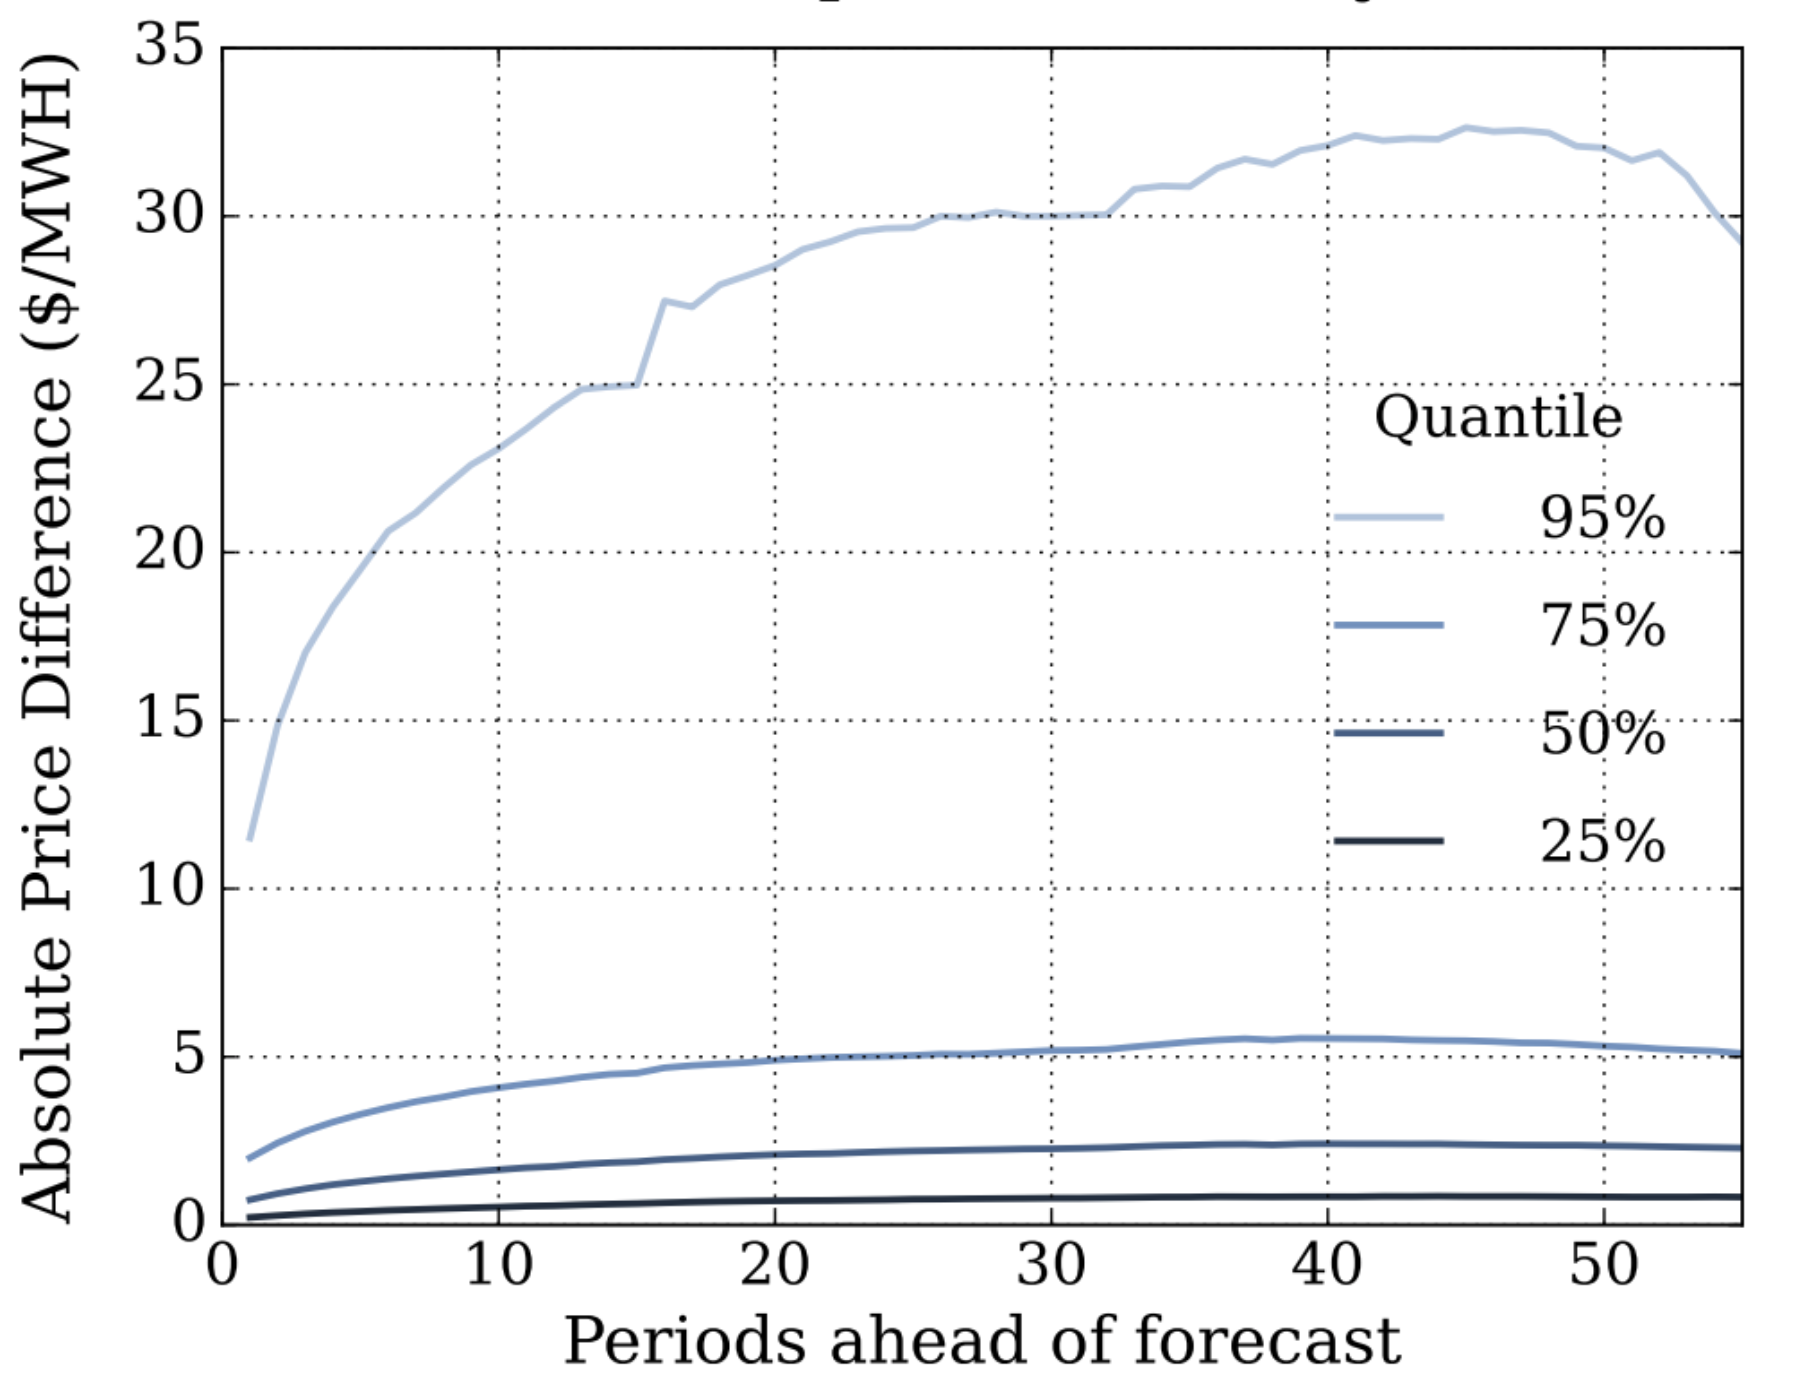
\includegraphics[width=0.5\textwidth]{Pictures/Chapter3/mcconnel_imperfect_forecast.png}
    \end{center}
    \caption{Pre-dispatch forecast accuracy. Periods ahead of forecast vs. absolute price difference, South Australia 2014 (McConnell 2014)}
    \label{fig:mcconnell_predispatch_accuracy}
\end{wrapfigure}
Although Chapter \ref{sec:energy_arbitrage} highlights the dynamics of battery energy storage, the results are theoretical and only place an \textbf{upper-bound} on energy arbitrage revenue. A  variety of approaches have been proposed for incorporating
imperfect foresight in electricity markets. \parencite{Sioshansi} used a ‘back casting’ approach, based on historic prices for the previous two weeks. \parencite{Wang} employed a `dynamic control algorithm' based on the following 24 hr ahead NEM pre-dispatch price forecasts (P30). \parencite{Wang} captured 60-85\% of the perfect foresight results for different states in the NEM in 2010, and noticed that it dropped to 20-50\% of the perfect foresight revenue in 2013. As previously highlighted in Figure \ref{fig:mcconnel_2014}, McConnell similarly used predispatch forecast prices, and using data from South Australia (2013-2014) found that increasing the storage improves the realisation of potential arbitrage value, from 70\% at 3 h to over 90\% at 8h. McConnell argues that this arises due to increased flexibility of the storage device. The ability to re-evaluate and change operation may be constrained for smaller devices.
\section{ AEMO Predispatch Forecast Accuracy }
\subsection{ P30 Predispatch Forecast  }
In McConnell's analysis, he highlighted ``\textit{More sophisticated analysis of predispatch pricing would further improve the value captured using pre-dispatch prices than the simple approach used here.}" McConnell provided elementary analysis of predispatch price accuracy as seen in Figure \ref{fig:mcconnell_predispatch_accuracy}.
\newline
This thesis similar to Wang and McConnell utilises the P30 forecast provided by AEMO. In other to understand BESS revenue under imperfect foresight, a comprehensive investigation into the accuracy of the P30 forecast has been undertaken.
\subsection{P30 Accuracy Method}
To analyse the accuracy of the P30 forecasts, a simple, yet data intensive methodology was undertaken. 
\begin{enumerate}
    \item Fetch P30 Data from AEMO NemWeb (from 2013 - 2018). This data includes 6 years of 30 minute forecasts with a variable time horizon spanning between 28 intervals (14 hrs) up to 79 intervals (39.5 hrs). For 5 states, this includes approx. \textbf{40 million} rows of data. 
    \item For each forecast determine the number of forecasts periods ahead (i.e. DATETIME - RUN\_DATETIME)
    \item For each forecast, determine the actual price which occured (RRP)
    \item Determine the relative error of each price forecast:
    \begin{equation}
        \text{Percentage Error (\%)} = \dfrac{100 \times (FORECAST\_RRP - RRP)}{RRP}
    \end{equation}
    \item Group predispatch data by region and number of predispatch forecast periods and determine the percentage error for quantiles in [5, 25, 50, 75, 95]  
\end{enumerate}
\subsection{P30 Accuracy - Summary of Results}
Appendix A contains the results of the P30 Analysis shown in Figures A.1 to A.5 for NSW, SA, QLD, VIC and TAS for years 2013 - 2016. Note these Figures are a 2D representation of Figure \ref{fig:predispatch_surface}.
\begin{wrapfigure}{r}{0.6\textwidth}
    \begin{center}
    \centering
    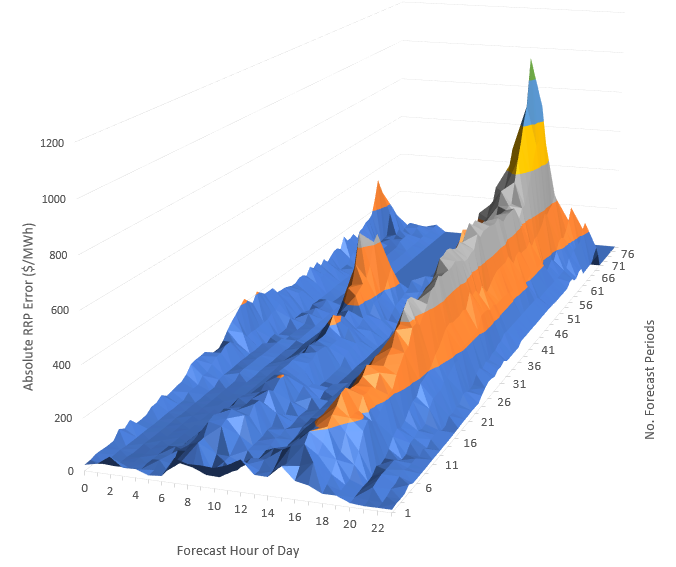
\includegraphics[width=0.6\textwidth]{Pictures/Chapter4/sa_forecast_error_2018.png}
    \end{center}
    \caption{Average Pre-dispatch forecast Absolute Error (\$/MWh) for South Australia, 2018}
    \label{fig:predispatch_surface}
\end{wrapfigure}
\subsubsection{Forecasting Improvement As Dispatch Near}
As shown in all the Figures in Appendix A, there is a clear convergence in price error as the dispatch period approaches i.e. as predispatch forecast periods approach 1. It is important to note that forecast periods greater than 60 typically represent forecasts for the early hours in the morning. The decrease in error beyond 50-60 periods ahead an artefact of the variable time horizon forecast. To illustrate this point, Figure \ref{fig:predispatch_surface} shows the absolute forecast errors for South Australia in 2018. The relationship where forecast error increases with number forecasts periods is particularly evident morning and evening peaks. Once strategy which could be employed to enhance revenue is to truncate the P30 forecast to only include the price forecast for the following 12 hours.
\newpage
\subsubsection{Forecast Accuracy Degradation}
In Appendix A, all states have exhibited a deterioration in price forecast accuracy, excluding QLD. As discussed in Chapter 3, the Queensland government `cracked down' on generator re-bidding and gaming the market in mid-2018. No-doubt this has been a contributing factor in the improvement in forecast accuracy in QLD from 2017- 2018. NSW and VIC have exhibited a similar characteristic ranging with percentage forecast error ranging from +/- 10\% range into the +100/-50\% range. This is really substantial for valuation of battery storage as price forecast which will inform short-term dispatch strategies are degrading year-on-year.
\subsubsection{Over Forecasting Evident}
Figures A.1 to A.6 typically show an over forecasting bias. This is especially evident in South Australia (Figure A.2), clearly displaying an asymmetric distribution of price error. This phenomenon may be likely to occur as AEMO typically over estimates demand for all regions \parencite{Madafiglio}.  
\section{ Energy Arbitrage with Imperfect Foresight Methodology }
To implement the energy arbitrage with imperfect foresight, a feedback loop is required, as seen in Figure \ref{fig:feedback_loop}.
\begin{figure}[H]
    \centering
    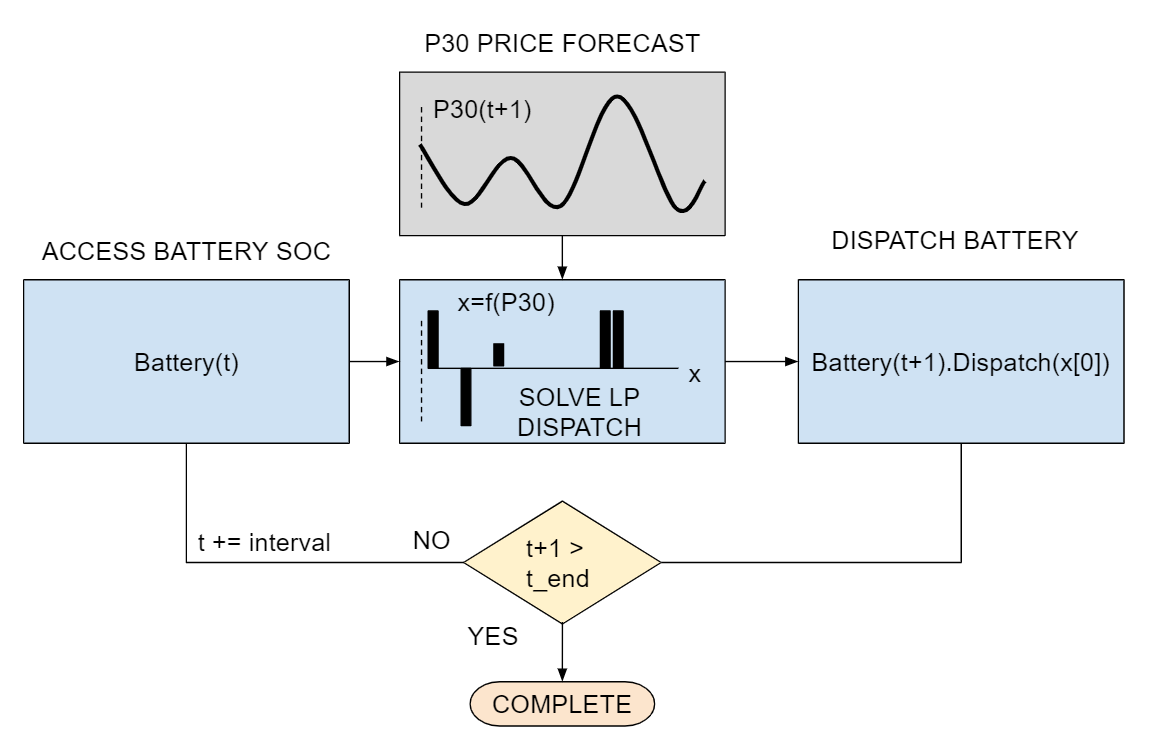
\includegraphics{Pictures/Chapter4/feedback_loop.png}
    \caption{Energy Arbitrage with Imperfect Foresight - Feedback Loop Methodology}
    \label{fig:feedback_loop}
\end{figure}
As seen in Figure \ref{fig:feedback_loop} to simulate a \textit{real battery} which doesn't have perfect foresight of price, the P30 forecast is used to inform the dispatch for the following time-step. Ultimately this requires the linear program to run each time step of the simulation period. It is important to note that this method does not represent actual dispatch and doesn't exhibit bidding characteristics in  5 minute market which settles under a 30 minute trading interval as seen in the NEM. 
Given the inter-temporal nature of this problem where SOC must be calculated at time-step (t) before proceeding to calculate SOC at time step (t+1), these simulations cannot be paralysed on multiple CPU cores or batch-ran.  To combat lengthy simulation time, at high-speed virtual machine on Google Cloud was utilised \url{https://cloud.google.com/compute/}. Google Cloud offers \$300 free credit for any Google Account. 
\section{ Validation }
Below Figure \ref{fig:2014_imperfect_mcconncel} shows the revenue captured by energy arbitrage for a BESS with 1 to 8 hours of storage. Figure \ref{fig:2014_imperfect} is the output of the imperfect foresight model. Both Figures demonstrate very similar characteristics, however Figure \ref{fig:2014_imperfect} has slightly higher perfect foresight revenue. This is attributed to the fact the models used in this thesis assume a round-trip efficiency of 81\%, however McConnell employed a 75\% round-trip efficiency. Despite these discrepancies this validates the imperfect foresight model. 
\begin{center}
\begin{figure}[H]
  \caption{FY 2014 - BESS Arbitrage Revenue, Perfect vs. Imperfect Foresight - McConnell (2015)}
  \label{fig:2014_imperfect_mcconncel}
  \centering
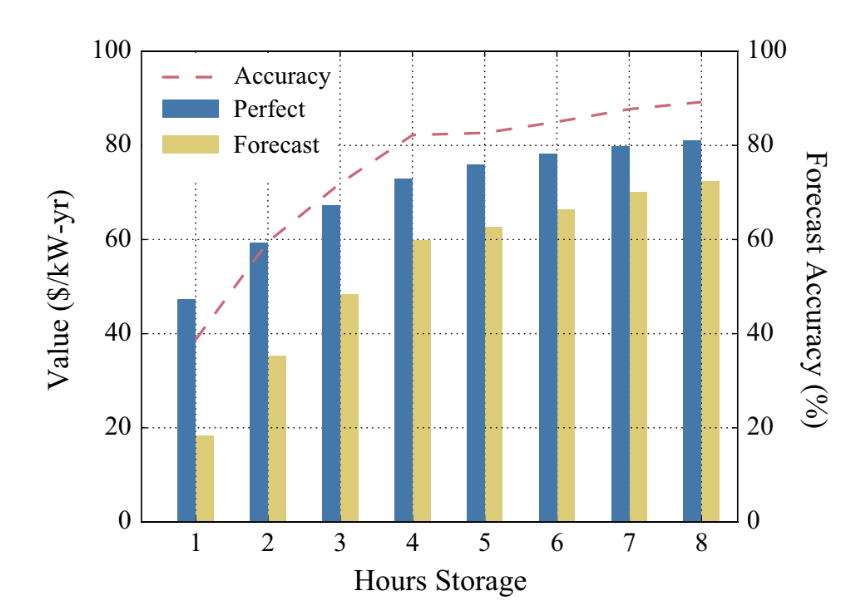
\includegraphics[width=0.7\textwidth]{Pictures/Chapter4/2014_Comp_McCon.png}
\end{figure}
\begin{figure}[H]
  \caption{FY 2014 - BESS Arbitrage Revenue, Perfect vs. Imperfect Foresight }
  \label{fig:2014_imperfect}
  \centering
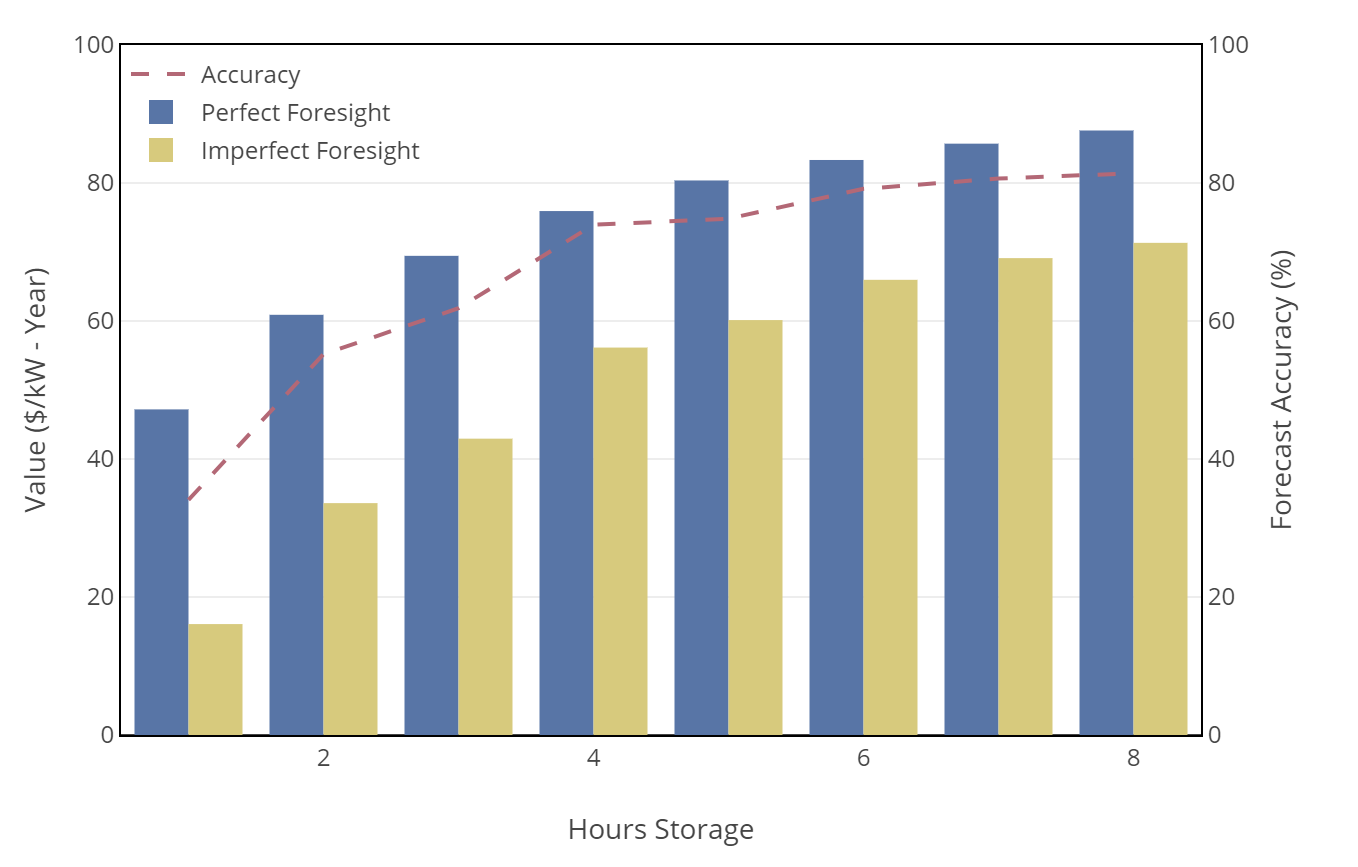
\includegraphics[width=0.7\textwidth]{Pictures/Chapter4/2014_Comp.png}
\end{figure}
\end{center}
\section{Results}
\foreach \x in {NSW, QLD, SA,VIC, TAS}
{ \begin{figure}[H]
  \caption{\x \; BESS Arbitrage Revenue, Perfect vs. Imperfect Foresight }
  \centering
  \hspace*{-2cm}
\includegraphics[width=1.1\textwidth]{"Pictures/Chapter4/Perfect Forecast vs Imperfect BESS Energy Arbitrage Revenue \x".pdf}
\end{figure}}
\subsection{Discussion}
\subsubsection{NSW}
New South Wales has exhibited an enormous increase in opportunity in BESS revenue. From 2013 to 2018, imperfect foresight BESS revenue has almost increased by \textbf{3 times}. The jump in revenue occurred in 2015, likely due to the privatisation of state owned generation businesses was completed in 2015 \parencite{AECOM}. As a result,
private entities own most generation capacity in NSW. AGL Energy (29 per cent), Origin Energy (23 per cent) and Snowy Hydro (19 per cent)
emerged as the state’s leading generators.
\subsubsection{Queensland}
As previously highlighted in Figure \ref{fig:generator_gaming}, Queensland has endured incredible volatility due to generator bidding games from 2013-2017. The introduction of \textit{Powering Queensland Plan} with the directive for Stanwell Corporation to undertake strategies to place downward pressure on wholesale prices, clearly made an impact in 2018. This is also supported by the fact forecast accuracy improved significantly from 2017 to 2018 (which usually deteriorates due to late generator rebidding). 
\subsubsection{ South Australia}
South Australia is the highest performer out of all the states, with the peak year in 2016. What is crucial to note in South Australia (2017) is that diminishing returns for additional hours of storage occur from 3 hours on-wards. On other words, \textbf{2 hours of storage is optimal}. This phenomenon arises as the additional storage grants the battery flexibility and enables capturing value from a price spike, even if the initial forecast was incorrect.
\subsubsection{ Victoria }
Victoria, naturally exhibits a cross between the characteristics of NSW and SA. Victoria has witnessed a gradual increase in BESS arbitrage value. This is likely to continue to increase after high price events have continued in Victoria in 2019, notably the heatwave in Victoria on March 1st 2019 \url{http://www.wattclarity.com.au/articles/2019/03/price-volatility-in-vic-and-sa-on-friday-1st-march/}.
\begin{wrapfigure}{r}{0.6\textwidth}
    \begin{center}
    \centering
    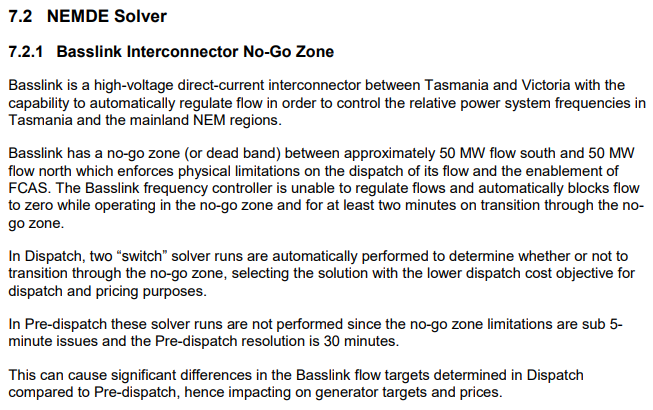
\includegraphics[width=0.6\textwidth]{Pictures/Chapter4/basslink.png}
    \label{fig:basslink_actual}
    \caption{Factors contributing to differences between Dispatch and Pre-dispatch outcomes: Basslink Interconnector (AEMO, 2018)}
    \end{center}
\end{wrapfigure}
\subsubsection{Tasmania}
Last and definitely least, Tasmania is a catastrophic state for battery storage using the P30 forecast. As shown in Figure A.5 South Australia has a tendency to over forecast price, consistently with a high degree of error. As highlighted by (AEMC, 2018), in Tasmania, rebidding is 65\% of the price spike cost. Furthermore, rebidding costs have increased by
165\% since 2015. Additionally, AEMO recognises that there are issues surrounding constraint accuracy in the P30 forecast, affecting the P30 price forecast for Tasmania. A detailed explanation of this issue is provided in Figure \ref{fig:basslink_actual}.
